\documentclass[aspectratio=169]{beamer}

\usepackage{basileabeam}
\usepackage[most]{tcolorbox}
\usepackage{subfig}


\setbeamercovered{invisible}
\addbibresource{presentation.bib}
% Notes:
%\pgfpagesuselayout{2 on 1}[a4paper,border shrink=5mm]
%\setbeamertemplate{note page}[plain]
%\setbeameroption{show notes on second screen=bottom}

\title              {Application of Graph Learning to inverse problems}

\author     		{Cédric Mendelin}
\email				{cedric.mendelin@stud.unibas.ch}
\institute          {Department of Mathematics and Computer Science, University of Basel}

\date               {09.12.2021}

\ulogo        		{Template/header}
\ulistelement    	{Template/listelement}

\graphicspath{{Figures/}}

% Options:
%\totalNoSlidesDisabled % To turn off the total number of slides in the footer. Comment this if you want the total number of slides in the footer

%\headerSectionsDisabled % Comment this if you want a fancy header containing your sections.


\begin{document}

\AtBeginSection[]{%
  \frame<beamer>{ 
    \frametitle{Outline}   
    \tableofcontents[currentsection] 
  }
}

\begin{frame}[t,plain]
    \titlepage
\end{frame}

\begin{frame}[t]{Outline}
    \tableofcontents
\end{frame}


%% Presentation content

\section{Imaging methods}	% You can also have slides prior to the first section or work entirely without sections.

\begin{frame}[c]{Cryo-electron microscopy (cryo-EM)}
    \begin{columns}[c]
        \column{.65\textwidth}
            \begin{itemize}
                \item Allows observation of molecules in near atomic resolution.
                \item Samples are frozen and further observed in electron microscope.
                \item During freezing, molecules rotate randomly.
                \item Frozen molecules are fragile, electron microscope needs to work with low power.
                \item Observations can be reconstructed to 3D model.
            \end{itemize}

            \begin{tcolorbox}[colback=red!5!white,hide=<-1>, alert=<2>, colframe=red!75!black]
                Only single particle cryo-EM is considered.
            \end{tcolorbox}
        \column{.35\textwidth}
        \begin{figure}
            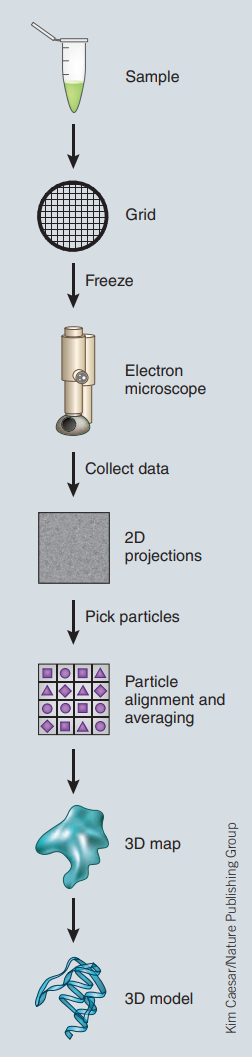
\includegraphics[width=0.22\textwidth]{cryo-em-workflow.png}
            \caption{Cryo-EM workflow \cite[Figure]{singleParticleCryoEm}}
        \end{figure}
    \end{columns}
\end{frame}

\begin{frame}[c]{Cryo-EM}
    \begin{figure}
        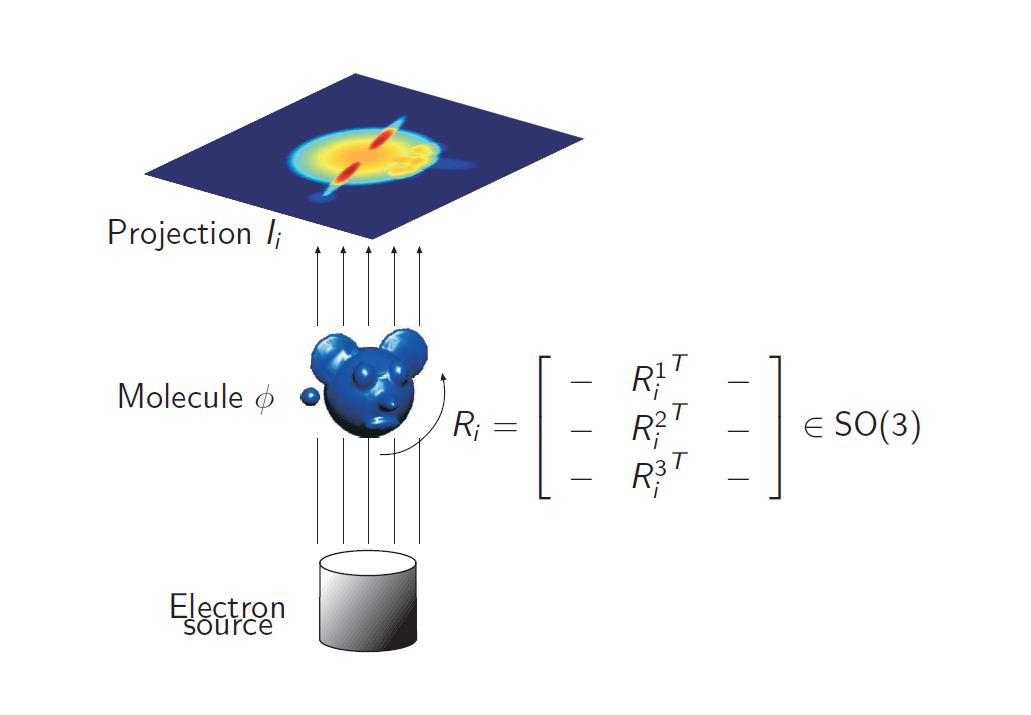
\includegraphics[width=0.4\textwidth]{cryo-EM-overview.png}
        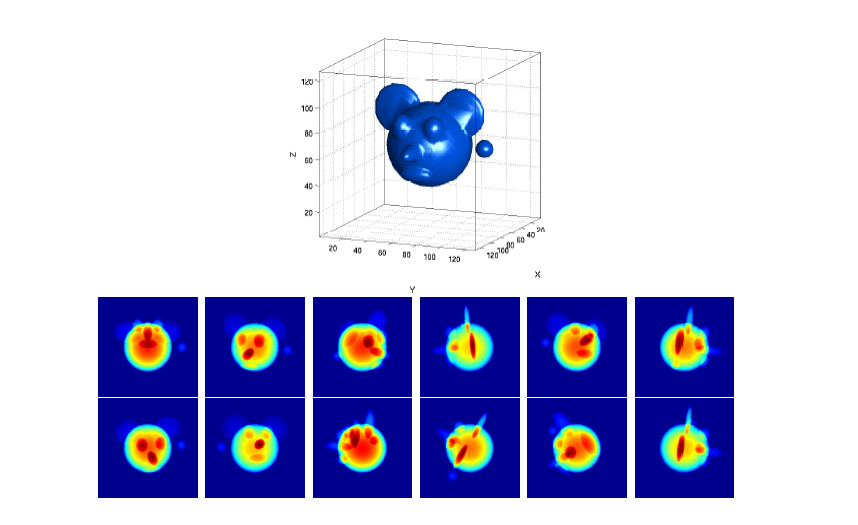
\includegraphics[width=0.4\textwidth]{micky-mouse.png}
        \caption{Cryo-EM overview \cite[Figure 1 and Figure 2]{cryoEmMath2}}
    \end{figure}

\end{frame}

\begin{frame}[c]{Cryo-EM challenges}
    \begin{columns}[c]
        \column{.50\textwidth}
        
        \begin{itemize}
            \item High-noise level 
            \item Unknown rotation during freezing
            \item (Structural variety of observations)
        \end{itemize}

        \begin{tcolorbox}[colback=red!5!white,hide=<-1>, alert=<2>,colframe=red!75!black]
            Master Thesis domain of interest is to high-noise regime (cryo-EM).
            Goal is to introduce a denoise method for cryo-EM 2D projections.
        \end{tcolorbox}

        \column{.50\textwidth}
        \begin{figure}
            \centering
            \subfloat[Noiseless photograph]
                {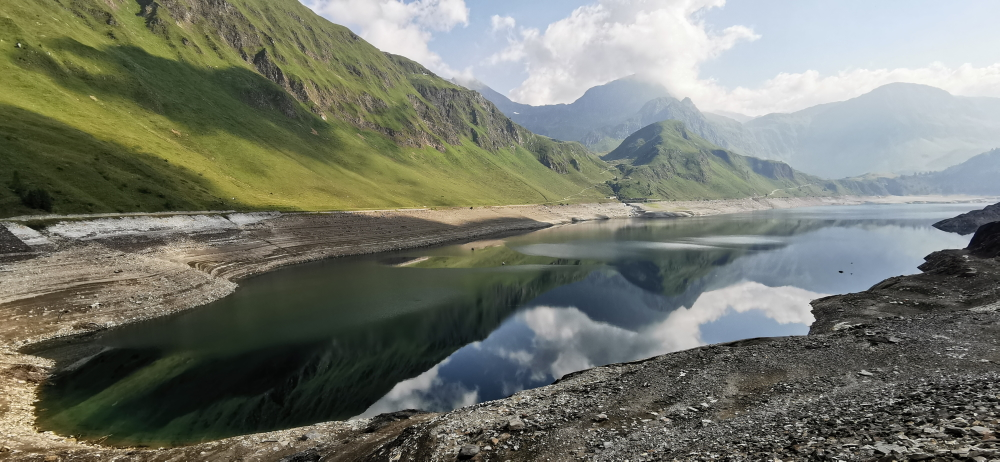
\includegraphics[width=0.6\textwidth]{rotom}} \\
            \subfloat[Noisy photograph]
                {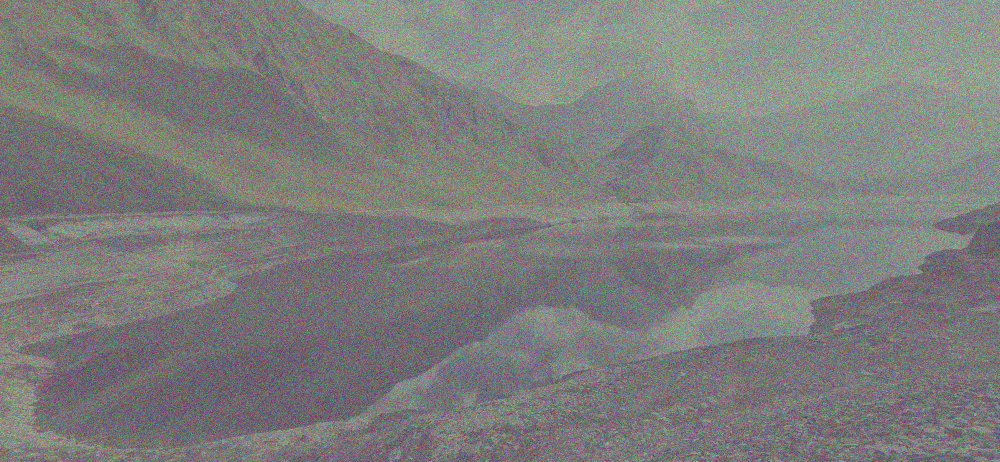
\includegraphics[width=0.6\textwidth]{rotom_noise}}
            \caption{Noise observation example}
        \end{figure}

    \end{columns}

    %\footnotetext[1]{https://www.ebi.ac.uk/emdb/EMD-32177}
\end{frame}

%\begin{frame}
%    \begin{definition}[Cryo-EM observation]
%        $$ y_i[j,k] = \Pi_z (\; Rot(\;x; \theta_i))_{j,k} + \eta_i[j,k], \text{ with } 1 \leq i \leq N \text{ and } 1 \leq j,k \leq M,$$
%    \end{definition}
%    \begin{itemize}
%        \item $y_i[] \in \tilde{\Omega}, x \in L^2(\Omega)$ with $\Omega \subset \mathbb{R}^3 $ and $\tilde{\Omega} \subset \mathbb{R}^2 $
%        \item $M$ observation dimension
%        \item $\Pi_z : L^2(\Omega) \to L^2(\tilde{\Omega})$ projection operator
%        \item $Rot : L^2(\Omega) \to L^2(\Omega),$ is rotation operator
%        \item $Rot(x, \theta_i) = \left((x_1,x_2,x_3) \mapsto x( x_1R^1_{\theta_i}, x_2R^2_{\theta_i}, x_3R^3_{\theta_i})\right)$
%        \begin{itemize}
%            \item $\theta_i = [\theta_i^{(1)}, \theta_i^{(2)}, \theta_i^{(3)} ] $, with $\theta_i^{(1)}, \theta_i^{(2)}, \theta_i^{(3)} \in \mathbb{R}$
%            \item $R_{\theta_i} =  [R^1_{\theta_i}, R^2_{\theta_i}, R^3_{\theta_i}] \in SO(3)$ is the 3D rotation matrix 
%        \end{itemize}
%    \end{itemize}
%\end{frame}


\begin{frame}[c]{Computed Tomography}
    \begin{columns}[c]
        \column{.55\textwidth}
            \begin{itemize}
                \item Related to cryo-EM
                \item Can be seen as simpler version in 2D
                \item Good to start with
            \end{itemize}
        
        \column{.45\textwidth}
            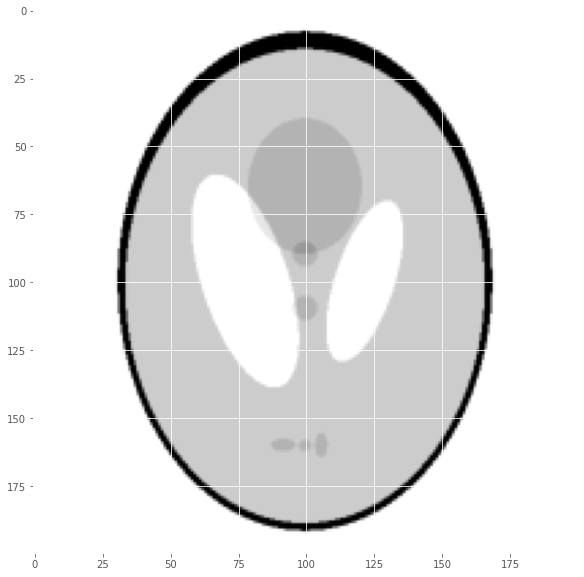
\includegraphics[width=0.4\textwidth]{phantom.png}
            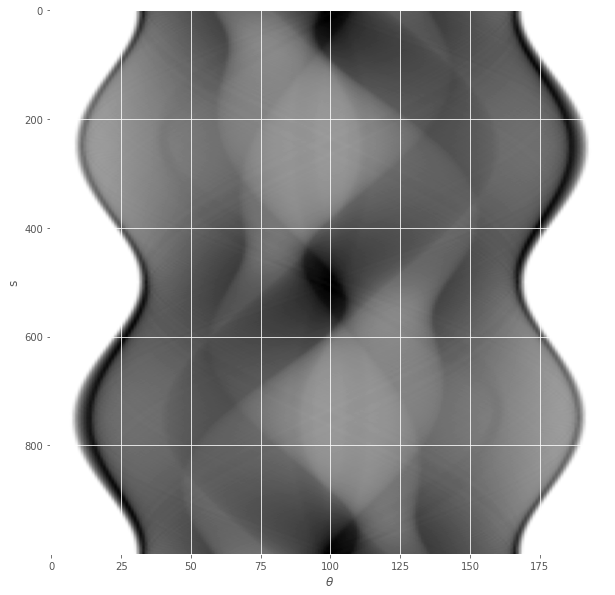
\includegraphics[width=0.4\textwidth]{phantom_sinogram.png}
                
        
    \end{columns}

\end{frame}

% \begin{frame}
%     \begin{definition}[CT observation]
%         $$ y_i[j] = R(x, \theta_i, s_j) + \eta_i[j] , \text{ with } 1 \leq i \leq N \text{ and } 1 \leq j \leq M,$$
%     \end{definition}
% 
%     \begin{itemize}
%         \item 
%     \end{itemize}
%     
% \end{frame}


\section{Graph Denoising}

\begin{frame}{Graph construction}
    Consider $n$ observed images $(x_0, x_1, \dots, x_n)$, where $x_i \in \mathbb{R}^M$ with $M$ as image dimension.
    A graph can be constructed by:
    \begin{itemize}
        \item $V$: Images can be used as nodes.
        \item $E$: If similarity measure \textbf{$d$} of two images $x_i, x_j$ is smaller than given threshold \textbf{$\tau$}, there will be an edge.
     \end{itemize}

     \pause
     \begin{definition}[Adjacency Matrix]
        \begin{equation}
            \label{eq:graphConstruction}
            A_{ij} =    
            \begin{cases}
                1  & \text{if } d(x_i, x_j) < \tau\\
                0, & \text{otherwise}
            \end{cases}
        \end{equation}
    \end{definition}
\end{frame}

\begin{frame}{Graph construction}
    Consider $n$ observed \textbf{noisy} images $(y_0, y_1, \dots, y_n)$, where $y_i \in \mathbb{R}^M$ with $M$ as image dimension.
    Then, $y_i = x_i + \eta$ with $\eta$ drawn from $\mathcal{N} \sim (0, \sigma^2)$ and $(x_0, x_1, \dots, x_n)$
    as the original images.
    A noisy graph can be constructed like:
    \begin{itemize}
        \item $V$: \textbf{Noisy} images $y$ can be used as nodes.
        \item $E$: If similarity measure $d$ of two \textbf{noisy} images $y_i, y_j$ is smaller than given threshold $\tau$, there will be an edge.
     \end{itemize}

     \pause

     \begin{definition}[Noisy Adjacency Matrix]
        \begin{equation}
            \label{eq:graphConstructionNoise}
            A_{0_{ij}} =    
            \begin{cases}
                1  & \text{if } d(y_i, y_j) < \tau\\
                0, & \text{otherwise}
            \end{cases}
        \end{equation}    
     \end{definition}
\end{frame}

%\begin{frame}[c]{Noisy graph}
%
%    \begin{definition}
%        For every noisy graph $G_0 = \langle V, E_0 \rangle$, 
%        there exists a noiseless graph $G = \langle V, E \rangle$.
%        Both graphs consists of the same set of vertices $V$ but different edges.
%        $E_0$  is defined as follows:
%        $$E_0 = E \setminus  E^{-}_0 \cup  E^{+}_0,$$
%        where $E^{-}_0 \subseteq E$ and $E^{+}_0 \subseteq U$ with $U$ the set of all possible edges and $E^{+}_0 \cap E = \emptyset$
%    \end{theorem}
%
%\end{frame}

\begin{frame}[c]{Graph Denoising}
    \textit{Graph denoising} is the task, to estimate a denoised graph $\tilde{G}$  
    from a given noisy graph $G_0$, with underlying original graph $G$:

    \begin{definition}[Graph Denoising]
        $$GD: G_0 \mapsto \tilde{G} \approx G,$$
    \end{definition}
    where $G_0$, $\tilde{G}$, $G$ denotes noisy, estimated denoised and original graph respectively.
   

\end{frame}

\section{Conclusion}

\begin{frame}[c]{Abstract model without noise}
    \begin{definition}[Noiseless observation abstract model]
        $$y_i = A(x, \theta_i), \text{ with } 1 \leq i \leq N ,$$
    \end{definition}

    \begin{itemize}
        \item $\Omega \subset \mathbb{R}^D$ as original object space with dimension $D$
        \item $\tilde{\Omega} \subset \mathbb{R}^{D-1}$ as observations space with dimension $D-1$.
        \item $y_i \in \tilde{\Omega}^M$ with $M$ observation dimension
        \item $x \in L^2(\Omega)$
        \item $\theta_i \in \mathbb{R}^P$ projection angle vector with projection dimension $P$
        \item $A: L^2(\Omega) \to L^2(\tilde{\Omega}), x \mapsto A(x; \theta_i)$, a non-linear operator  
    \end{itemize}

\end{frame}

\begin{frame}[c]{Computed tomography - low-dimensional manifold}
    \begin{columns}
        \column{.55\textwidth}
        \begin{itemize}
            \item Observations $y_i$  with angle $\theta_i$
            \item There is a mapping between observation $y_i$ and $\theta_i$
            \item For computed tomography, $\theta \in [0, 2\pi]$ (circle)
            \item Therefore, there exists a one to one mapping from $y_i$ to points on the circle.
        \end{itemize}
        
        \column{.55\textwidth}
        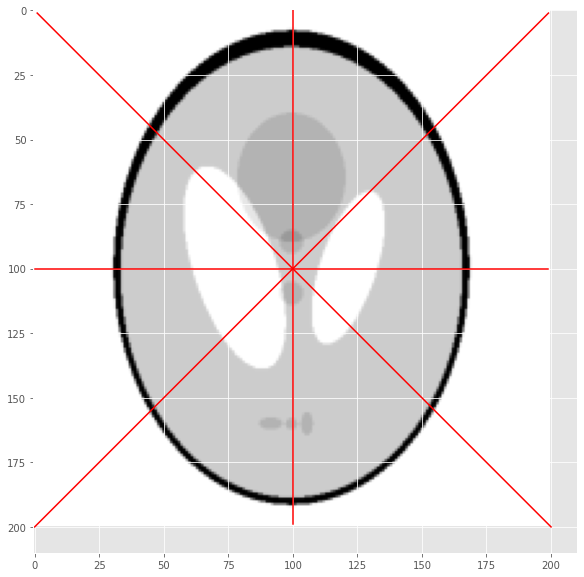
\includegraphics[width=0.6\textwidth]{phantom_many_theta.png}
        
    \end{columns}
\end{frame}


\begin{frame}[c]{Manifolds}
    We know structure of manifolds for noiseless data:
    \begin{itemize}
        \item Computed Tomography $\to$ circle
        \item Cryo-Em $\to$ sphere
    \end{itemize}

    If data is noisy, manifold will "drift" away from noiseless manifold:
    \begin{figure}
        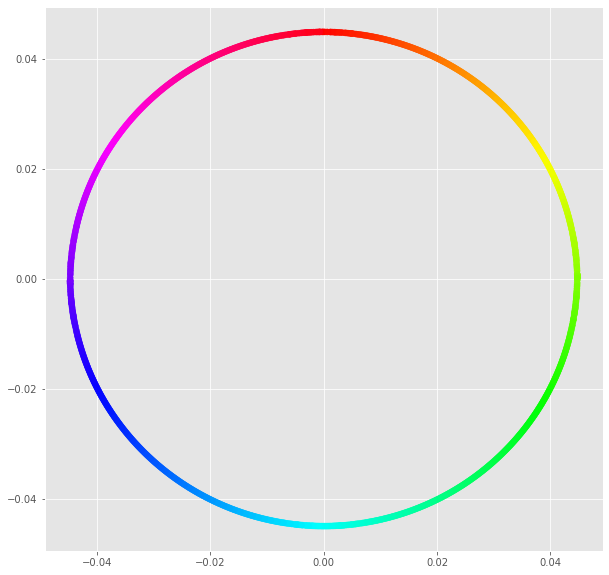
\includegraphics[width=0.2\textwidth]{phantom_second_third_evec}
        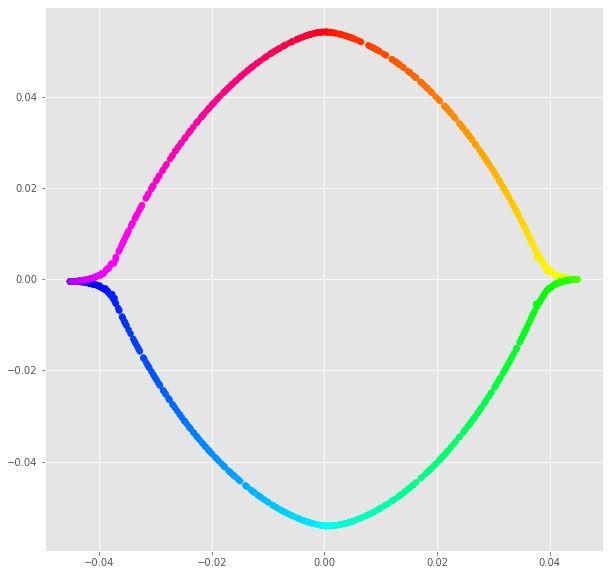
\includegraphics[width=0.2\textwidth]{phantom_second_third_evec_noisy}
        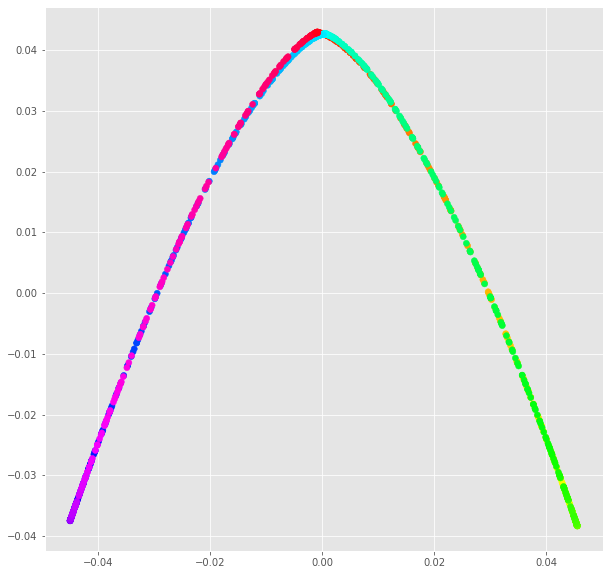
\includegraphics[width=0.2\textwidth]{phantom_second_third_evec_noisy2}
        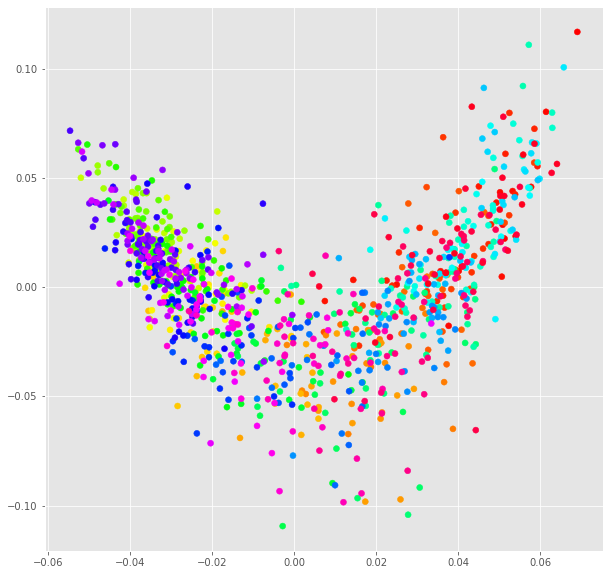
\includegraphics[width=0.2\textwidth]{phantom_second_third_evec_noisy_high}
        \caption{Manifolds for phantom without noise, and different noise levels.}
    \end{figure}
\end{frame}


\begin{frame}{Project Conclusion - Next steps}
    \begin{itemize}
        \item Focus on high-noise domain (cryo-EM)
        \item Introduce Graph Denoising method
        \item Exploit known manifold in 2D and 3D
        \item Further study Graph Laplacian and connection with
            \begin{itemize}
                \item Tomography domain
                \item GNNs and Machine Learning in general
            \end{itemize}
        \item Evaluate on toy dataset in 2D and 3D
        \item Nice to have: evaluate on cryo-EM / CT dataset
    \end{itemize}
\end{frame}

\begin{frame}{Project schedule}
    \begin{figure}
        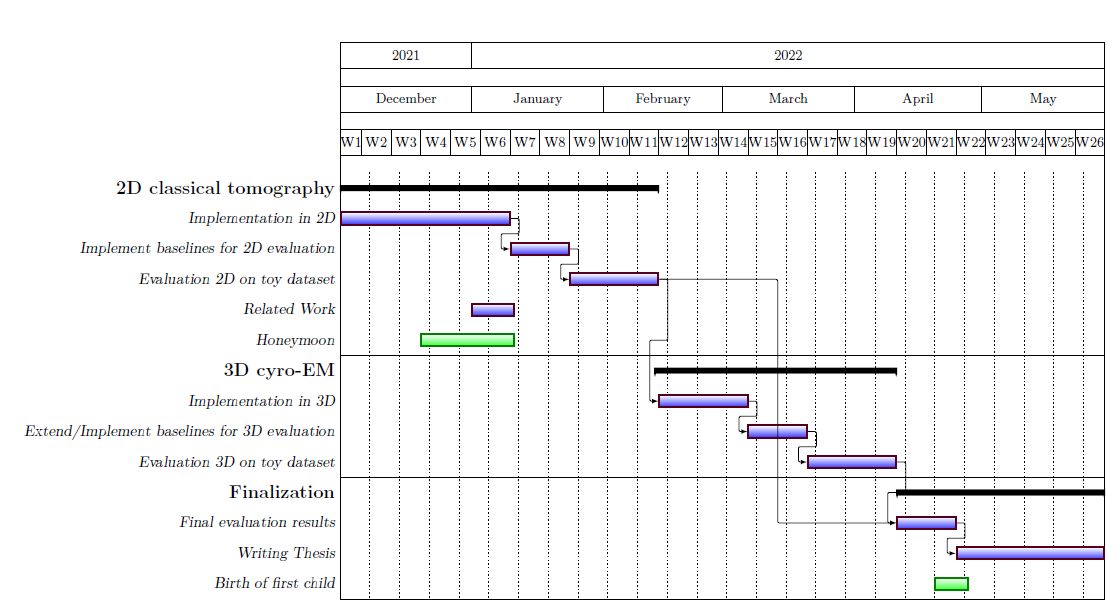
\includegraphics[width=0.8\textwidth]{gantt_chart}
    \end{figure}
\end{frame}

\begin{frame}[t,plain]
\lastpage{{\usebeamerfont{title} Questions?}\\[5ex]}
\end{frame}

\backupbegin

\begin{frame}{References}
    \printbibliography
\end{frame}

\backupend

\end{document}

